\paragraph{}
RGL est un package pour le langage de programmation R. Il étend les possibilités de R avec l'ajout d'outils de visualisation 3D en temps réel.
\paragraph{}
Les univers 3D ont besoin d’être projetées sur des images 2D affichées à l’écran, c'est pourquoi il est nécessaire d'avoir un outils qui effectue cette étape afin d'afficher des objets tri-dimensionnel à l’écran. Cet outils doit simuler la lumière, la structure des objets et leurs textures afin de donner l'illusion de 3D sur les images 2D projetées.
\begin{center}
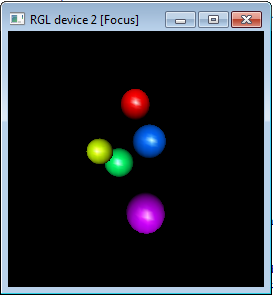
\includegraphics[scale=0.7]{screen_rgl2.png}\\
\textit{Des sphères dans RGL}
\end{center}


\paragraph{}
Le coeur de RGL est codé en c++ et utilise OpenGL. RGL est ainsi une interface entre R et OpenGL. OpenGL est un standard des applications graphiques utilisé dans un grand nombre d'applications et langages. Il résout notamment le problème d'affichage en 2D d'univers 3D cité plus tôt. 
\paragraph{}
Plusieurs fonctionnalités sont accessibles simultanément via RGL, telles que l’intégration drag/drop dans la fenêtre de visualisation et la réception de nouvelles instructions depuis la console de commande de R. Ainsi les objets peuvent être examinés en trois-dimension grâce au zoom et la scène peut pivoter sur elle-même.

\begin{center}
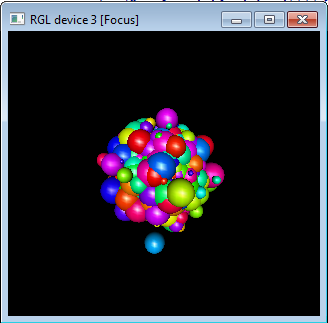
\includegraphics[scale=0.7]{screen_rgl3.png}\\
\textit{Plus de sphères dans RGL}
\end{center}


\paragraph{}
Le but de RGL est donc de surcoucher OpenGL pour le langage R. Il permet ainsi via des instruction en R de générer des scènes 3D et d'interagir avec celles-ci via de nombreux outils.
